\documentclass[10pt, french]{article}

%% -----------------------------
%% Préambule
%% -----------------------------
% !TEX encoding = UTF-8 Unicode
% LaTeX Preamble for all cheatsheets
% Author : Gabriel Crépeault-Cauchon

% HOW-TO : copy-paste this file in the same directory as your .tex file, and add in your preamble the next command right after you have specified your documentclass : 
% \input{preamble-cheatsht.tex}
% ---------------------------------------------
% ---------------------------------------------

% Extra note : this preamble creates document that are meant to be used inside the multicols environment. See the documentation on internet for further information.

%% -----------------------------
%% Encoding packages
%% -----------------------------
\usepackage[utf8]{inputenc}
\usepackage[T1]{fontenc}
\usepackage{babel}
\usepackage{lmodern}

%% -----------------------------
%% Variable definition
%% -----------------------------
\def\auteur{Gabriel Crépeault-Cauchon / Nicholas Langevin}
\def\BackgroundColor{white}

%% -----------------------------
%% Margin and layout
%% -----------------------------
% Determine the margin for cheatsheet
\usepackage[landscape, hmargin=1cm, vmargin=1.7cm]{geometry}
\usepackage{multicol}

% Remove automatic indentation after section/subsection title.
\setlength{\parindent}{0cm}

% Save space in cheatsheet by removing space between align environment and normal text.
\usepackage{etoolbox}
\newcommand{\zerodisplayskips}{%
  \setlength{\abovedisplayskip}{0pt}%
  \setlength{\belowdisplayskip}{0pt}%
  \setlength{\abovedisplayshortskip}{0pt}%
  \setlength{\belowdisplayshortskip}{0pt}}
\appto{\normalsize}{\zerodisplayskips}
\appto{\small}{\zerodisplayskips}
\appto{\footnotesize}{\zerodisplayskips}

%% -----------------------------
%% URL and links
%% -----------------------------
\usepackage{hyperref}
\hypersetup{colorlinks = true, urlcolor = gray!70!white, linkcolor = black}

%% -----------------------------
%% Document policy (uncomment only one)
%% -----------------------------
%	\usepackage{concrete}
	\usepackage{mathpazo}
%	\usepackage{frcursive} %% permet d'écrire en lettres attachées
%	\usepackage{aeguill}
%	\usepackage{mathptmx}
%	\usepackage{fourier} 

%% -----------------------------
%% Math configuration
%% -----------------------------
\usepackage[fleqn]{amsmath}
\usepackage{amsthm,amssymb,latexsym,amsfonts}
\usepackage{empheq}
\usepackage{numprint}
\usepackage{dsfont} % Pour avoir le symbole du domaine Z

% Mathematics shortcuts

\newcommand{\reels}{\mathbb{R}}
\newcommand{\entiers}{\mathbb{Z}}
\newcommand{\naturels}{\mathbb{N}}
\newcommand{\eval}{\biggr \rvert}
\usepackage{cancel}
\newcommand{\derivee}[1]{\frac{\partial}{\partial #1}}
\newcommand{\prob}[1]{\Pr \left( #1 \right)}
\newcommand{\esp}[1]{\mathrm{E} \left[ #1 \right]} % espérance
\newcommand{\variance}[1]{\mathrm{Var} \left( #1   \right)}
\newcommand{\covar}[1]{\mathrm{Cov} \left( #1   \right)}
\newcommand{\laplace}{\mathcal{L}}
\newcommand{\deriv}[2][]{\frac{\partial^{#1}}{\partial #2^{#1}}}
\newcommand{\e}[1]{\mathrm{e}^{#1}}
\newcommand{\te}[1]{\text{exp}\left\{#1\right\}}
\DeclareMathSymbol{\shortminus}{\mathbin}{AMSa}{"39}



% To indicate equation number on a specific line in align environment
\newcommand\numberthis{\addtocounter{equation}{1}\tag{\theequation}}

%
% Actuarial notation packages
%
\usepackage{actuarialsymbol}
\usepackage{actuarialangle}

%
% Matrix notation for math symbols (\bm{•})
%
\usepackage{bm}
% Matrix notation variable (bold style)
\newcommand{\matr}[1]{\mathbf{#1}}



%% -----------------------------
%% tcolorbox configuration
%% -----------------------------
\usepackage[most]{tcolorbox}
\tcbuselibrary{xparse}
\tcbuselibrary{breakable}

%%
%% Coloured box "definition" for definitions
%%
\DeclareTColorBox{definition}{ o }				% #1 parameter
{
	colframe=blue!60!green,colback=blue!5!white, % color of the box
	breakable, 
	pad at break* = 0mm, 						% to split the box
	title = {#1},
	after title = {\large \hfill \faBook},
}
%%
%% Coloured box "definition2" for definitions
%%
\DeclareTColorBox{definitionNOHFILL}{ o }				% #1 parameter
{
	colframe=blue!60!green,colback=blue!5!white, % color of the box
	pad at break* = 0mm, 						% to split the box
	title = {#1},
	before title = {\faBook \quad },
	breakable
}


%%
%% Coloured box "algo" for algorithms
%%
\newtcolorbox{algo}[ 1 ]
{
	colback = blue!5!white,
	colframe = blue!75!black,
	title=#1,
	fonttitle = \bfseries,
	breakable
}
%%
%% Coloured box "conceptgen" for points adding to a concept's deifintion
%%
\newtcolorbox{conceptgen}[ 1 ]
{
	breakable,
	colback = beaublue,
	colframe = airforceblue,
	title=#1,
	fonttitle = \bfseries
}
%%
%% Coloured box "probch3" pour formules relatives au 3ème chapitre de prob
%%
\newtcolorbox{probch3}[ 1 ]
{
	colback = ruddypink,
	colframe = burgundy,
	fonttitle = \bfseries,	
	breakable,
	title=#1
}
%%
%% Coloured box "formula" for formulas
%%
\newtcolorbox{formula}[ 1 ]
{
	colback = green!5!white,
	colframe = green!70!black,
	breakable,
	fonttitle = \bfseries,
	title=#1
}
%%
%% Coloured box "formula" for formulas
%%
\DeclareTColorBox{algo2}{ o }
{
	enhanced,
	title = #1,
	colback=blue!5!white,	
	colbacktitle=blue!75!black,
	fonttitle = \bfseries,
	breakable,
	boxed title style={size=small,colframe=arsenic} ,
	attach boxed title to top center = {yshift=-3mm,yshifttext=-1mm},
}
%%
%% Coloured box "examplebox" for formulas
%%
\newtcolorbox{examplebox}[ 1 ]
{
	colback = lightmauve,
	colframe = antiquefuchsia,
	breakable,
	fonttitle = \bfseries,title=#1
}
%%
%% Coloured box "rappel" pour rappel de formules
%%
\newtcolorbox{rappel}[ 1 ]
{
	colback = ashgrey,
	colframe = arsenic,
	breakable,
	fonttitle = \bfseries,title=#1
}
%%
%% Coloured box "rappel" pour rappel de formules
%%
\DeclareTColorBox{rappel_enhanced}{ o }
{
	enhanced,
	title = #1,
	colback=ashgrey, % color of the box
%	colframe=blue(pigment),
%	colframe=arsenic,	
	colbacktitle=arsenic,
	fonttitle = \bfseries,
	breakable,
	boxed title style={size=small,colframe=arsenic} ,
	attach boxed title to top center = {yshift=-3mm,yshifttext=-1mm},
}
%%
%% Coloured box "notation" for notation and terminology
%%
\DeclareTColorBox{distributions}{ o }			% #1 parameter
{
	enhanced,
	title = #1,
	colback=gray(x11gray), % color of the box
%	colframe=blue(pigment),
	colframe=arsenic,	
	colbacktitle=aurometalsaurus,
	fonttitle = \bfseries,
	boxed title style={size=small,colframe=arsenic} ,
	attach boxed title to top center = {yshift=-3mm,yshifttext=-1mm},
	breakable
%	left=0pt,
%  	right=0pt,
%    box align=center,
%    ams align*
%  	top=-10pt
}

%% -----------------------------
%% Graphics and pictures
%% -----------------------------
\usepackage{graphicx}
\usepackage{pict2e}
\usepackage{tikz}

%% -----------------------------
%% insert pdf pages into document
%% -----------------------------
\usepackage{pdfpages}

%% -----------------------------
%% Color configuration
%% -----------------------------
\usepackage{color, soulutf8, colortbl}


%
%	Colour definitions
%
\definecolor{blue(munsell)}{rgb}{0.0, 0.5, 0.69}
\definecolor{blue(matcha)}{rgb}{0.596, 0.819, 1.00}
\definecolor{blue(munsell)-light}{rgb}{0.5, 0.8, 0.9}
\definecolor{bleudefrance}{rgb}{0.19, 0.55, 0.91}
\definecolor{blizzardblue}{rgb}{0.67, 0.9, 0.93}
\definecolor{bondiblue}{rgb}{0.0, 0.58, 0.71}
\definecolor{blue(pigment)}{rgb}{0.2, 0.2, 0.6}
\definecolor{bluebell}{rgb}{0.64, 0.64, 0.82}
\definecolor{airforceblue}{rgb}{0.36, 0.54, 0.66}
\definecolor{beaublue}{rgb}{0.74, 0.83, 0.9}
\definecolor{cobalt}{rgb}{0.0, 0.28, 0.67}	% nice light blue-ish
\definecolor{blue_rectangle}{RGB}{83, 84, 244}		% ACT-2004
\definecolor{indigo(web)}{rgb}{0.29, 0.0, 0.51}	% purple-ish
\definecolor{antiquefuchsia}{rgb}{0.57, 0.36, 0.51}	%	pastel dark purple ish
\definecolor{darkpastelpurple}{rgb}{0.59, 0.44, 0.84}
\definecolor{gray(x11gray)}{rgb}{0.75, 0.75, 0.75}
\definecolor{aurometalsaurus}{rgb}{0.43, 0.5, 0.5}
\definecolor{ruddypink}{rgb}{0.88, 0.56, 0.59}
\definecolor{pastelred}{rgb}{1.0, 0.41, 0.38}		
\definecolor{lightmauve}{rgb}{0.86, 0.82, 1.0}
\definecolor{azure(colorwheel)}{rgb}{0.0, 0.5, 1.0}
\definecolor{darkgreen}{rgb}{0.0, 0.2, 0.13}			
\definecolor{burntorange}{rgb}{0.8, 0.33, 0.0}		
\definecolor{burntsienna}{rgb}{0.91, 0.45, 0.32}		
\definecolor{ao(english)}{rgb}{0.0, 0.5, 0.0}		% ACT-2003
\definecolor{amber(sae/ece)}{rgb}{1.0, 0.49, 0.0} 	% ACT-2004
\definecolor{green_rectangle}{RGB}{131, 176, 84}		% ACT-2004
\definecolor{red_rectangle}{RGB}{241,112,113}		% ACT-2004
\definecolor{amethyst}{rgb}{0.6, 0.4, 0.8}
\definecolor{amethyst-light}{rgb}{0.6, 0.4, 0.8}
\definecolor{ashgrey}{rgb}{0.7, 0.75, 0.71}			% dark grey-black-ish
\definecolor{arsenic}{rgb}{0.23, 0.27, 0.29}			% light green-beige-ish gray
\definecolor{amaranth}{rgb}{0.9, 0.17, 0.31}
\definecolor{brickred}{rgb}{0.8, 0.25, 0.33}
\definecolor{pastelred}{rgb}{1.0, 0.41, 0.38}

%
% Useful shortcuts for coloured text
%
\newcommand{\orange}{\textcolor{orange}}
\newcommand{\red}{\textcolor{red}}
\newcommand{\cyan}{\textcolor{cyan}}
\newcommand{\blue}{\textcolor{blue}}
\newcommand{\green}{\textcolor{green}}
\newcommand{\purple}{\textcolor{magenta}}
\newcommand{\yellow}{\textcolor{yellow}}

%% -----------------------------
%% Enumerate environment configuration
%% -----------------------------
%
% Custum enumerate & itemize Package
%
\usepackage{enumitem}
%
% French Setup for itemize function
%
\frenchbsetup{StandardItemLabels=true}
%
% Change default label for itemize
%
\renewcommand{\labelitemi}{\faAngleRight}


%% -----------------------------
%% Tabular column type configuration
%% -----------------------------
\newcolumntype{C}{>{$}c<{$}} % math-mode version of "l" column type
\newcolumntype{L}{>{$}l<{$}} % math-mode version of "l" column type
\newcolumntype{R}{>{$}r<{$}} % math-mode version of "l" column type
\newcolumntype{f}{>{\columncolor{green!20!white}}p{1cm}}
\newcolumntype{g}{>{\columncolor{green!40!white}}m{1.2cm}}
\newcolumntype{a}{>{\columncolor{red!20!white}$}p{2cm}<{$}}	% ACT-2005
% configuration to force a line break within a single cell
\usepackage{makecell}


%% -----------------------------
%% Fontawesome for special symbols
%% -----------------------------
\usepackage{fontawesome}

%% -----------------------------
%% Section Font customization
%% -----------------------------
\usepackage{sectsty}
\sectionfont{\color{\SectionColor}}
\subsectionfont{\color{\SubSectionColor}}

%% -----------------------------
%% Footer/Header Customization
%% -----------------------------
\usepackage{lastpage}
\usepackage{fancyhdr}
\pagestyle{fancy}

%
% Header
%
\fancyhead{} 	% Reset
\fancyhead[L]{Aide-mémoire pour~ \cours ~(\textbf{\sigle})}
\fancyhead[R]{\auteur}

%
% Footer
%
\fancyfoot{}		% Reset
\fancyfoot[R]{\thepage ~de~ \pageref{LastPage}}
\fancyfoot[L]{\href{https://github.com/ressources-act/Guide_de_survie_en_actuariat}{\faGithub \ ressources-act/Guide de survie en actuariat}}
%
% Page background color
%
\pagecolor{\BackgroundColor}




%% END OF PREAMBLE
% ---------------------------------------------
% ---------------------------------------------
%% -----------------------------
%% Variable definition
%% -----------------------------
\def\cours{Introduction à l'actuariat II}
\def\sigle{ACT-2001}
\def\SectionColor{burntorange}
\def\SubSectionColor{burntsienna}
\def\SubSubSectionColor{burntsienna}

%% Reduce margin space
\setlength{\abovedisplayskip}{-15pt}
\setlist{leftmargin=*}

\newcommand{\bettershortstack}[2][c]{%
  \begin{tabular}[b]{@{}#1@{}}#2\end{tabular}%
}
\usepackage{stackengine}
\newcommand\cumlaut[2][black]{\stackon[.33ex]{#2}{\textcolor{#1}{\kern-.04ex.\kern-.2ex.}}}
%% -----------------------------
%% Début du document
%% -----------------------------
\begin{document}

\begin{center}
	\textsc{\Large Contributeurs}\\[0.5cm] 
\end{center}
%\input{contributeurs/contrib-ACT2001}

\newpage

\raggedcolumns
\begin{multicols*}{2} 

\section{Terminologie}
\begin{description}
	\item[$\argmax$]	Si on pose que $\hat{\theta}	=	\argmax L(\theta; \bm{X})$ on dit que la valeur maximale de $L(\theta; \bm{X})$ est au point $\hat{\theta}$.
\end{description}

Paramètre
\begin{description}
%%%	https://www.statisticshowto.com/shape-parameter/
	\item[de forme]	Affecte la forme générale de la distribution;
		\begin{itemize}
		\item	\og \textit{shape parameter} \fg{};
		\item	Il est important de saisir que le paramètre de forme n'a aucune incidence sur l'emplacement de la densité (paramètre de l'emplacement) ni sur l'échelle de la densité (paramètre d'échelle);
		\item	Par exemple, la distribution Gamma a un paramètre de forme qui impact comment qu'elle est représentée;
		\item	Par exemple, la distribution exponentielle n'a pas de paramètre de forme et bien que l'échelle de la distribution peut être modifiée, la forme générale est constante.
		\end{itemize}
%%%		
	\item[d'échelle]	Sert à déterminer la forme et l'emplacement de la distribution en étirant ou compressant la densité;
		\begin{itemize}
		\item	\og \textit{scale parameter} \fg{};
		\item	Le plus gros le paramètre d'échelle, le plus rependue la distribution;
		\item	On peut voir ceci visuellement où avec un paramètre d'échelle de 1, la distribution est inchangée:
		\end{itemize}
		\begin{center}
\tikzset{every picture/.style={line width=0.75pt}} %set default line width to 0.75pt        

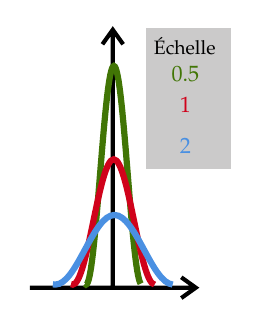
\begin{tikzpicture}[x=0.75pt,y=0.75pt,yscale=-1,xscale=1]
%uncomment if require: \path (0,300); %set diagram left start at 0, and has height of 300

%Shape: Axis 2D [id:dp18693685040272978] 
\draw [line width=1.5]  (119.83,151.67) -- (199.83,151.67)(159.83,27.4) -- (159.83,151.67) (192.83,146.67) -- (199.83,151.67) -- (192.83,156.67) (154.83,34.4) -- (159.83,27.4) -- (164.83,34.4)  ;
%Shape: Wave [id:dp5641937191696826] 
\draw  [color={rgb, 255:red, 65; green, 117; blue, 5 }  ,draw opacity=1 ][line width=2.25]  (146.41,149.77) .. controls (146.59,150.04) and (146.77,150.18) .. (146.95,150.18) .. controls (149.38,150.18) and (151.47,124.5) .. (153.66,97.51) .. controls (155.85,70.53) and (157.94,44.84) .. (160.37,44.84) .. controls (162.8,44.84) and (164.89,70.53) .. (167.08,97.51) .. controls (169.1,122.49) and (171.05,146.35) .. (173.25,149.77) ;
%Shape: Wave [id:dp9736357574926828] 
\draw  [color={rgb, 255:red, 208; green, 2; blue, 27 }  ,draw opacity=1 ][line width=2.25]  (139.7,149.94) .. controls (139.97,150.1) and (140.23,150.18) .. (140.5,150.18) .. controls (144.08,150.18) and (147.17,135.46) .. (150.39,119.99) .. controls (153.62,104.52) and (156.71,89.8) .. (160.29,89.8) .. controls (163.87,89.8) and (166.96,104.52) .. (170.19,119.99) .. controls (173.38,135.28) and (176.43,149.85) .. (179.96,150.18) ;
%Shape: Wave [id:dp9806953027168039] 
\draw  [color={rgb, 255:red, 74; green, 144; blue, 226 }  ,draw opacity=1 ][line width=2.25]  (130.98,150.05) .. controls (131.36,150.14) and (131.74,150.18) .. (132.12,150.18) .. controls (137.28,150.18) and (141.73,142) .. (146.38,133.41) .. controls (151.03,124.82) and (155.48,116.64) .. (160.64,116.64) .. controls (165.8,116.64) and (170.25,124.82) .. (174.9,133.41) .. controls (179.4,141.74) and (183.72,149.68) .. (188.68,150.16) ;
%Shape: Rectangle [id:dp4682062525043522] 
\draw  [draw opacity=0][fill={rgb, 255:red, 203; green, 202; blue, 202 }  ,fill opacity=1 ] (176,26.67) -- (216.83,26.67) -- (216.83,94.67) -- (176,94.67) -- cycle ;

% Text Node
\draw (178.42,29.67) node [anchor=north west][inner sep=0.75pt]  [font=\scriptsize,color={rgb, 255:red, 0; green, 0; blue, 0 }  ,opacity=1 ] [align=left] {Échelle};
% Text Node
\draw (186.92,43.67) node [anchor=north west][inner sep=0.75pt]  [font=\footnotesize,color={rgb, 255:red, 65; green, 117; blue, 5 }  ,opacity=1 ] [align=left] {0.5};
% Text Node
\draw (190.92,58.67) node [anchor=north west][inner sep=0.75pt]  [font=\footnotesize,color={rgb, 255:red, 208; green, 2; blue, 27 }  ,opacity=1 ] [align=left] {1};
% Text Node
\draw (190.92,78.67) node [anchor=north west][inner sep=0.75pt]  [font=\footnotesize,color={rgb, 255:red, 74; green, 144; blue, 226 }  ,opacity=1 ] [align=left] {2};


\end{tikzpicture}
		\end{center}
	\item[de fréquence]	L'interprétation dépend du contexte.
		\begin{itemize}
		\item	\og \textit{rate parameter} \fg{};
		\item	Dans le cas d'un processus de Poisson, le paramètre de fréquence décrit le taux auquel les événements se produisent;
		\item	Souvent, il est défini comme le réciproque du paramètre d'échelle pour indiquer le taux de déclin d'une fonction exponentielle;
		\item	Des valeurs près de 1 impliquent un déclin lent alors que des valeurs près de 0 impliquent un déclin rapide.
		\end{itemize}
%%%		https://www.statisticshowto.com/location-parameter/
	\item[d'emplacement]	Stipule où la densité est située.
		\begin{itemize}
		\item	\og \textit{location parameter} \fg{};
		\item	Plus précisément, indique où sur l'axe des $x$ la distribution est centrée relatif à la distribution normale standard;
		\item	Une distribution normale standard est centrée à 0 donc un paramètre d'emplacement de 5 implique que la densité est centrée à $x	=	5$.
		\end{itemize}
\end{description}


\begin{distributions}[Notation]
\begin{description}
	\item[$S$]	Les coûts d'un portefeuille.
	\item[$\rho(S)$]	Une mesure de risque.
\end{description}
\end{distributions}

\section{Mesures de risque}

\begin{description}
	\item[Capital économique]	Allocation de surplus de la compagnie;
		\begin{align*}
		CE(S)	
		&=	\rho(S)	-	\esp{S}
		\end{align*}
	\item[Marge de risque]	associée à une prime $P(X)$;
		\begin{align*}
		MR(X)
		&=	\rho(X)	-	\esp{X}
		\end{align*}
\end{description}

$\rho$ introduit une marge de risque:
\begin{description}
	\item[positive]	lorsque \icbox{$\rho(X)	\geq		\esp{X}$} pour une v.a. $X$ avec \icbox[red][palechestnut]{$\esp{X} < \infty$};
	\item[justifiée]	lorsque \icbox{$\rho(X)	=	\rho(a)	=	a$} pour une v.a. $X$ avec \icbox[red][palechestnut]{$\Pr(X	=	a)	=	1, \alpha > 0$};
	\item[non-excessive]	lorsque \icbox{$\rho(X)	\leq		a_{\max}$} pour une v.a. $X$ \icbox[red][palechestnut]{s'il existe $a_{\max}	<	\infty$} \icbox[red][palechestnut]{tel que $\Pr(X	\leq		a_{\max})	=	1$};
\end{description}

\subsection{Propriétés désirables d'une mesure de risque}
\begin{definitionNOHFILLsub}[Homogénéité]
Soit une v.a. $X$ et un scalaire \icbox[red][palechestnut]{$c	>	0$}, la mesure de risque $\rho$ est dite homogène si \icbox{$\rho(cX)	=	c\rho(X)$}.
\end{definitionNOHFILLsub}

\begin{definitionNOHFILLsub}[Invariance à la translation]
Soit une v.a. $X$ et un scalaire \icbox[red][palechestnut]{$c	\in	\mathbb{R}$}, la mesure de risque $\rho$ satisfait la propriété d'invariance à la translation si \icbox{$\rho(X + c)	=	\rho(X) + c$}.	\\

Ajouter un montant positif à un risque ajoute un montant équivalent à la mesure de risque.
\end{definitionNOHFILLsub}

\begin{definitionNOHFILLsub}[Monotonicité]
Soit les v.a. $X_{1}$ et $X_{2}$ \icbox[red][palechestnut]{tel que $\Pr(X	\leq	X_{2})	=	1$}, la mesure de risque $\rho$ satisfait la propriété de monotonicité si \icbox{$\rho(X_{1})	\leq	\rho(X_{2})$} ou si \icbox[red][palechestnut]{$\forall	u	\in	(0, 1)$}, \icbox{$F_{X_{1}}^{-1}(u)	\leq	F_{X_{2}}^{-1}(u)$}.

\end{definitionNOHFILLsub}

\begin{definitionNOHFILLsub}[Sous-additivité]
Soit les v.a. $X_{1}$ et $X_{2}$, la mesure de risque $\rho$ satisfait la propriété de sous-additivité si \icbox{$\rho(X_{1}	+	X_{2})	\leq	\rho(X_{1})	+	\rho(X_{2})$}.

\end{definitionNOHFILLsub}

\begin{definitionNOHFILLsub}[Convexité]
Soit les v.a. $X_{1}$ et $X_{2}$, la mesure de risque $\rho$ satisfait la propriété de convexité si \icbox{$\rho(\alpha X_{1}	+	(1	-	\alpha)X_{2})	\leq	\alpha\rho(X_{1})	+	(1	-	\alpha)\rho(X_{2})$}.

\end{definitionNOHFILLsub}

\subsection{TVaR et VaR}

\begin{itemize}
	\item	La \textbf{Value-at-Risk} correspond au $100\alpha^{\text{e}}$ pourcentile;
	\item	Si $X$ représente les gains, on s'intéresse à l'extrémité inférieure de la distribution des gains et \icbox{$TVaR_{\alpha}(X)	=	\esp{X | X \leq \alpha}	=	\frac{1}{\alpha} \int_{-\infty}^{VaR_{\alpha}} x f_{X}(x)dx$};
	\item	Si $X$ représente les pertes, on s'intéresse à l'extrémité supérieure de la distribution des gains et \icbox{$TVaR_{\alpha}(X)	=	\esp{X | X > \alpha}	=	\frac{1}{1 - \alpha} \int_{VaR_{\alpha}}^{\infty} x f_{X}(x)dx$};
\end{itemize}

\pagebreak

\section{Modèles de risques non-vie}
\begin{distributions}[Notation]
\begin{description}
	\item[$M$]	Variable aléatoire du nombre de sinistres pour un risque;
	\item[$B_{k}$]	Variable aléatoire du montant du $k^{\text{e}}$ sinistre.
\end{description}
\end{distributions}

\begin{definitionNOHFILL}[Modèle fréquence-sinistre]
On défini la v.a. $X$ comme étant les coûts (pertes) pour un risque tel que \icbox[red][palechestnut]{$\forall	M	>	0$}:
\begin{align*}
	X
	&=	\sum_{k	=	1}^{M} B_{k}
\end{align*}

\tcbline

\begin{align*}
	\esp{X}
	&=	\text{E}_{\text{M}}\left[\text{E}_{\text{B}}[X | M]\right]	\\
	&=	\text{E}[M]	\times	\text{E}[B]	\\
	\text{Var}(X)
	&=	\underbrace{\text{Var}_{\text{M}}(\text{E}_{\text{B}}[X | M])}_{\text{variabilité du \textit{nombre} de sinistres}}	+	\underbrace{\text{E}_{\text{M}}\left[\text{Var}_{\text{B}}(X | M)\right]}_{\text{variabilité du \textit{coût} par sinistre}}	\\
	&=	\text{E}[M]\text{Var}(B)	+	\text{E}^{2}[B]\text{Var}(M)	\\
\end{align*}

\tcbline

\begin{align*}
	F_{X}(x)
	&=	\Pr(M	=	0)	+	\sum_{k	=	1}^{\infty} \Pr(M	=	k)F_{B_{1}	+	\dots	+	B_{k}}(x)
\end{align*}

Par exemple, pour $B_{k}	\sim	\Gamma(\alpha,	\beta)$:
\begin{align*}
	F_{X}(x)
	&=	\Pr(M	=	0)	+	\sum_{k	=	1}^{\infty} \Pr(M	=	k)H(x;	\alpha k, \beta)
\end{align*}

\tcbline

\begin{align*}
	\mathcal{L}_{X}(t)
	&=	P_{M}\left(\mathcal{L}_{B}(t)\right), \quad	t > 0	\\
	\esp{X	\times	\bm{1}_{\{X	>	b\}}}
	&=	\sum_{k	=	1}^{\infty} \Pr(M	=	k)E\left[(B_{1}	+	\dots	+	B_{k})	\times	\bm{1}_{\{B_{1}	+	\dots	+	B_{k} > b\}}\right]
\end{align*}

Par exemple, pour $B_{k}	\sim	\Gamma(\alpha,	\beta)$:
\begin{align*}
	\esp{X	\times	\bm{1}_{\{X	>	b\}}}
	&=	\sum_{k	=	1}^{\infty} \Pr(M	=	k) \frac{k\alpha}{\beta} \overline{H}(b;	\alpha k + 1, \beta)
\end{align*}
\end{definitionNOHFILL}

\end{multicols*}
\end{document}

